\documentclass[aps,pra,10pt,twocolumn]{revtex4-2}
% revtex4-2 = version 2 of the review text class
% aps       = American Physical Society (society type)
% pra       = Physical Review A (journal type)
% 10pt      = font size
% twocolumn = true

\usepackage{silence} % NB: put *before* package you want to silence
\WarningFilter{caption}{Unknown document class} % Caption package does not support revtex4

\usepackage{times} % Times New Roman

\usepackage[a4paper, left=1.85cm, right=1.85cm,top=1.85cm, bottom=1.85cm]{geometry}

% Defines caption font size as 9pt and caption title bolded
\usepackage[style=base, font=small, labelfont=bf]{caption}
\usepackage{subcaption}

\usepackage{graphics,graphicx,epsfig,ulem}  % Graphics package
\usepackage{amsmath} 						% Maths package

\usepackage{siunitx} % SI units, alignment in tables

\usepackage{lipsum}
\usepackage[british]{babel} % British date system

\usepackage{multirow} % Multirow cells in tables
\usepackage{booktabs} % Nice table separators

\usepackage{hyperref} % For hyperreferences


% Customise date to preferred format
\usepackage{etoolbox}
\makeatletter
\patchcmd{\frontmatter@RRAP@format}{(}{}{}{}
\patchcmd{\frontmatter@RRAP@format}{)}{}{}{}
\renewcommand\Dated@name{}
\makeatother

\usepackage{fancyhdr}
\pagestyle{fancy}                           % Insert header
\renewcommand{\headrulewidth}{0pt}
\lhead{L.\ Kirby}                           % Header name
\rhead{Towards the automatic arrangement of music via quantum annealing}            % Header title              

\def\bibsection{\section*{References}}      % Defining bibsection
 
\begin{document}

\title{Towards the automatic arrangement of music via quantum annealing}
\author{L.\ Kirby}                              % Author
\affiliation{Durham University}                % Subtitle
\date{Submitted: \today{}}     % Date

\begin{abstract}              

\lipsum[1]

\end{abstract}

\maketitle

\thispagestyle{plain} % Produces front page number

\section{Introduction} 

Music is often seen as a very human endeavour.

Traditionally, the arrangement of music is a complex process that requires a deep understanding of musical theory, structure, and style. Composers use their creativity and intuition to create a piece that is both musically interesting and emotionally engaging, a challenging and often time-consuming process, requiring a great deal of skill and experience. Perhaps it is unsurprising, then, that there has been interest in automating this process.

One of the earliest examples of this can be seen in the \textit{Musikalisches Würfelspiel} ("musical dice game") system popular in the 18th century. The roll of dice would determine the order of pre-composed musical phrases, allowing for the creation of new music without the need for a composer. This system was engaged by the likes of Bach and Mozart, although fell out of fashion the following century.

The introduction of computers in the 20th century allowed for more sophisticated methods of music arrangement. Genetic algorithms and neural networks have been used to arrange music, with varying degrees of success. However, these methods are limited by the complexity of the problem and the need for extensive training data.

With the advent of quantum computers, there become growth in a new field of quantum computer music.

The combination of quantum computing and music is a relatively new field, but one that has shown promise. Quantum computers have the potential to solve complex optimisation problems that are intractable for classical computers, and music arrangement is one such problem.

Quantum computing comes in two flavours: gate-based and annealing. Gate-based quantum computers, such as those developed by IBM and Google, use quantum gates to manipulate qubits and perform calculations. Quantum annealers, such as those developed by D-Wave, use quantum fluctuations to find the global minimum of a given function. Each are suited to solving different classes of problems, with gate-based computers being more versatile and annealers being more efficient for certain optimisation problems. 

Computational complexity "One of the roles of computational complexity theory is to determine the practical limits on what computers can and cannot do". Quantum annealers are particularly well-suited to solving a class of problems known as NP-hard. A well-known example of an NP-hard problem is the travelling salesman problem, where the goal is to find the shortest route that visits a set of cities exactly once. This problem is difficult to solve because the number of possible routes grows exponentially with the number of cities. Quantum annealers have been shown to be effective at solving NP-hard problems, and have been used to find solutions to a variety of optimisation problems, such as protein folding [CITE], financial portfolio optimisation [CITE], and traffic flow optimisation [CITE].

This paper will focus on a subset of arrangement known as \textit{reduction}—taking a score written for a large number of parts and reducing it to a smaller number of parts, whilst still retaining the musicality and structure of the original. This is a common task in music production, where a piece written for a full orchestra may need to be arranged for a smaller ensemble, such as a string quartet. This forgoes the need to generate new music, as all notes in the arrangement are taken from the original score, and is more readily available to analyse as an optimisation problem. Quantum music generation is currently a developing field \cite{miranda_quantum_2022}, but beyond the scope of this paper. 

\section{Theory} 

Annealing, in metallurgical terms, is the process of heating and cooling a material to alter its physical properties. The cooling stage is typically slow to allow the material soften \cite{oed_annealing_2024}. In the context of quantum computing, quantum annealing is a computational technique that uses quantum fluctuations to find the global minimum of a given function. Much like its metallurgical counterpart, quantum annealing is a slow process that allows the system to settle into a low-energy state.

The system is first prepared in a ground state $H_0$, and then allowed to evolve to a second state $H_P$ according to
\begin{equation}
    H(t)=\left(1- \frac{t}{T}\right)H_0 + \frac{t}{T}H_P \,.
    \label{eq:time-evolution}
\end{equation}
If this is done adiabatically, with a sufficiently large $T$, the system will remain in the ground state of $H(t)$, and therefore end in the ground state of $H_P$. This is the principle of quantum annealing.

Quantum annealing can be used to solved combinatorial optimisation problems, which are problems that require the minimisation of a function over a discrete set of variables. If we prepare $H_P$ such that its ground state encodes the solution to the optimisation problem, then as long as $H_0$ and $H_P$ do not commute, the solution will be given at the end of the annealing process.



\section{Embedding}

The general form of a QUBO is
\begin{equation}
    f(x)=\sum_iQ_{i,i}x_i+\sum_{i<j}Q_{i,j}x_ix_j
    \label{eq:QUBO}
\end{equation}
where $Q$ is a coefficient matrix (??).

\section{Problem formulation}

Previous approaches to the automatic arrangement of music have been based on the use of genetic algorithms and neural networks. However, these methods are limited by the complexity of the problem and the need for extensive training data. In this study, we propose a new approach to the automatic arrangement of music based on quantum annealing.

It has been shown that the automatic arrangement of music can be formulated as a combinatorial optimisation problem \cite{moses_computational_2016}. Given a set of musical phrases, the goal is to find an optimal arrangement of these phrases such that the overall quality of the arrangement is maximised. This problem can be formulated as a maximum independent set (MIS) problem, which is a well-known optimisation problem. The MIS problem can then be solved using quantum annealing, which already has well-known QUBO formulations \cite{lucas_ising_2014}.

The maximum independent set (MIS) QUBO takes the form
\begin{equation}
    f(x)=A\sum_{ij\in E}x_ix_j-B\sum_i x_i
    \label{eq:MIS}
\end{equation}




%Identify most important results clearly and convincingly
%Shows that computer code works correctly (numerical convergences, systematic errors, random errors, etc.)

\begin{figure}[h]
    \centering
    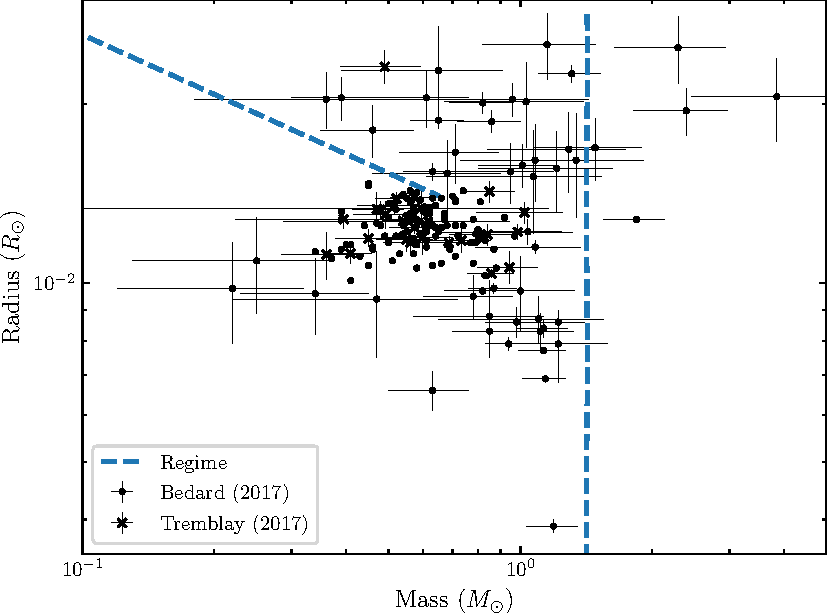
\includegraphics[width=\linewidth]{images/regime-model.pdf}
    \caption{}
    \label{fig:regime}
\end{figure}

% Physical implication of results
% Does code work? Comparison to literature, tests (IMPORTANT)
% Demonstrate student's contribution and motivation

\section{Method}

There are many formats that allow the digital manipulation of music, each with their own benefits, but this study primarily uses MusicXML \cite{musicxml}. This format focuses on the representation of standard sheet music, allowing for musical notes, rests, and other musical symbols, as well as the structure of the music, such as the arrangement of notes into measures (bars) and parts. It is widely supported by music notation software, allowing translation of music between graphic, textual, and audio formats.

Since interaction with the D-Wave QPUs is handled in Python, the surrounding manipulation of music is also written in this way. The module \verb|music21| provides extensive resources for manipulating, translating, and creating music, allowing scores to be broken down and reconstructed as fit.

A MusicXML file of the original score is first read into the program. The score is then broken down into its constituent parts, measures, and notes. Each note is represented by a vector of features, such as pitch and duration. The parts are then split into its musical phrases; these are identified via a local boundary detection model (LBDM). The phrases are numbered and a graph of the problem constructed, with each phrase as a node and edges between nodes representing the compatibility of phrases.

Phrases can be assigned a weighting based on their entropy. The entropy of a phrase can be seen as how much musical information it contains, with a higher entropy indicating a more complex phrase. Maximisation of phrase entropy can be used to create richer arrangements. For a random variable $X$ with a probability distribution $P(X)$, the entropy is defined as
\begin{equation}
    H(X)=-\sum_i P(x_i)\log_2 P(x_i)
    \label{eq:entropy}
\end{equation}
where each $x_i$ is a possible value of $X$. In this context, the random variable is a musical note, considering its possible values both in terms of pitch and rhythm.

Pitch entropy is calculated by considering the distribution of pitches in a phrase. The probabilities of each pitch $x_i$ can be found by
\begin{equation}
    P(x_i)=\frac{n_i}{N}
    \label{eq:pitch-prob}
\end{equation}
where $n_i$ is the number of times pitch $x_i$ appears in the phrase and $N$ is the total number of notes in the phrase.

Rhythm entropy is calculated in a similar way, but instead of considering the duration of notes, the inter-onset interval (IOI) is used instead. This is the time interval between the start of two consecutive notes, which is often more noticeable than the length of the notes themselves. This is also calculated using Eq.\ \ref{eq:pitch-prob}, but instead considering $x_i$ as possible IOI values.
The total entropy of a phrase is then the sum of the pitch and rhythm entropy over all its notes. 

Once the graph is formed, the MIS QUBO can be constructed and sent to the D-Wave QPU to be solved. The solutions returned will be sets of phrases that are compatible with each other and form the final arrangement. These can then be reconstructed into a new file which can be translated into sheet music or audio.

\begin{table}[ht] % Table environment specifies caption, label, location
    \caption{Summary of frational changes to best-fit parameters due to electron energy density and electrostatic corrections.}
    \label{tab:corrections}
    \setlength{\tabcolsep}{12pt} % Column spacing
    \renewcommand{\arraystretch}{1.5}
    \begin{tabular}{c|c|c|c} % S aligns to decimal point
        \toprule
        \textbf{Correction} & $|\Delta A|/A$ & $|\Delta B|/B$ & $|\Delta q|/q$\\
        \midrule
        $\varepsilon_\mathrm{elec}$ & 0.026 & 0.0031 & 0.0442 \\
        $p_c$ & 0.009 & 0.0114 & 0.0005 \\
        \bottomrule
    \end{tabular}
\end{table}

\section{Non-degenerate limit}

\begin{align}
    p&=\frac{\hbar c}{12\pi^2}\left(\frac{3\pi^2}{m_n c^2\eta}\right)^{4/3}\left[\frac{1+2d(S_e)^2+\frac{7}{15}d(S_e)^4}{(1+d(S_e)^2)^{4/3}}\right]\varepsilon^{4/3}\\
    &=\bar{K}(S_e)\varepsilon^{4/3} \,.
    \label{eq:nondegeos}
\end{align}

\section{Conclusions}

%Present ideas for further investigation

The study of white dwarfs is very much ongoing research, with new models arising with the advancement of computational power and new satellite observations that test these models. It is incredible that an investigation such as this, through the application of fundamental statistical physics and computer modelling, can attempt to understand the nature of stellar remnants that seem so unreachable.

\nocite{*}
\bibliographystyle{unsrt}\bibliography{interim}

\clearpage

\onecolumngrid % Puts summary into single column

\section*{Scientific Summary for a General Audience}

\lipsum[1]

\end{document}